%---------------------------------------------------------------------------%
%-                                                                         -%
%-                           LaTeX Template UPO                            -%
%-                                                                         -%
%---------------------------------------------------------------------------%

%---------------------------------------------------------------------------%
%->> Document class declaration
%---------------------------------------------------------------------------%

\documentclass[
A4paper,                % paper size A4
twoside,                % onesite or twoside printing
openany,              % doublepage cleaning ends up right side
chapterprefix=true,     % prefix for chapter marks
12pt,                   % font size
headings=normal,        % size of headings
titlepage=on            % own page for each title page
]{book}
\let\cleardoublepage\clearpage

%---------------------------------------------------------------------------%
%->> Document Details
%---------------------------------------------------------------------------%

\newcommand{\University}{\protect{Universidad Pablo de Olavide}}
\newcommand{\UNIVERSITY}{\protect{UNIVERSIDAD PABLO DE OLAVIDE}}

\newcommand{\thesisTitle}{\protect {<Title of the doctoral thesis>}}
\newcommand{\thesisAuthor}{\protect{<Name and Surnames>}}
\newcommand{\priorstudies}{\protect{<Previous academic degree>}}
\newcommand{\thesisDate}{<Year>}

\newcommand{\UPOCentre}{\protect {<Faculty name, not abbreviated>}}


\newcommand{\DoctoralProgramme}{\protect{<Name of the doctoral programme, not abbreviated>}}

\newcommand{\supervisor}{<Supervisor Name and Surnames> }
\newcommand{\cosupervisor}{<[Add co-supervisor if applicable]> }

\newcommand{\supervisorDetails}{<Supervisor Name and Surnames, position, institution> }
\newcommand{\cosupervisorDetails}{<[Add co-supervisor if applicable, including position and institution]> }

%---------------------------------------------------------------------------%
%->> Document Style and Settings
%---------------------------------------------------------------------------%

% **************************************************
% Settings
% **************************************************
% --------------------------
% Packages
% --------------------------
\usepackage[english]{babel}          % Multilingual support: English and Spanish, with Spanish-specific elements replaced
\usepackage[utf8]{inputenc}          % Allows input of special characters (e.g., accents, ñ) in UTF-8 encoding
\usepackage[T1]{fontenc}             % Use T1 font encoding for better handling of accented characters

\usepackage{mathpazo}                 % Use a similar version to Calibri

%\usepackage{mathptmx}                % Use a modern version of Times New Roman

%\usepackage{lmodern}                 % Use a modern, scalable font (Latin Modern), ensuring high-quality output
%\usepackage{palatino}               % Optional: use Palatino font instead of the default (commented out)

\usepackage[protrusion=true, expansion=true]{microtype}  % Improves typography with character protrusion and font expansion
\usepackage{amsmath,amssymb}         % Math packages for enhanced mathematical symbols and environments
\usepackage{tabularx}                % Create tables that automatically adjust column widths to fit the text width
\usepackage{multicol}                % Support for creating multi-column text within tables or documents
\usepackage{multirow}                % Allows for cells spanning multiple rows in tables
\usepackage{longtable}               % Create tables that can span multiple pages
\usepackage{booktabs}                % Enhances tables with professional-looking horizontal rules (toprule, midrule, etc.)
\usepackage{ltablex}                 % Combines `longtable` and `tabularx` features for flexible and multi-page tables
\usepackage{setspace}                % Provides control over line spacing (e.g., single, one-and-a-half, or double spacing)
\usepackage{tikz}                    % Powerful package for creating vector-based graphics and diagrams
\usetikzlibrary{fadings, calc}   % Load the fadings library to enable gradient fading effects
\usepackage{graphicx,graphics}       % Handles inclusion of images in the document
\usepackage{subfig}                  % Modern package for managing subfigures (replaces `subfigure`)
\usepackage{wrapfig}        % For wrapping text around figures
\usepackage[export]{adjustbox}       % Allows for alignment and scaling adjustments when including images
\usepackage{ragged2e}                % Provides commands for justified and ragged text alignment (e.g., `\RaggedRight`)
\usepackage{comment}                 % Allows for large blocks of text to be commented out
\usepackage{blindtext}               % Generates dummy text for testing purposes (e.g., `\blindtext`)
\usepackage[acronym,nonumberlist,nomain,hyperfirst=true]{glossaries}  % Manages lists of acronyms (without numbering or main glossary)
\usepackage[hidelinks]{hyperref}     % Adds clickable hyperlinks in the document without colored boxes or borders
\usepackage[a4paper]{geometry}       % Sets the document margins and page size (configured for A4 paper)
\usepackage{parskip}                 % Controls paragraph spacing, typically disabling indentation and adding space between paragraphs
\usepackage{fancyhdr,everypage}      % Customizes headers and footers throughout the document
\usepackage{enumitem}                % Provides control over the formatting of lists (e.g., itemize, enumerate)
\usepackage{color}                   % Basic color support for text/elements
\usepackage[dvipsnames,table]{xcolor} % Adds color support (specifically for tables and named colors like `dvipsnames`)
\usepackage{emptypage}               % Ensures that empty pages do not display headers or footers
\usepackage{caption}  % Customizes caption appearance (e.g., small font, hanging indent, bold labels)
\usepackage{subcaption}              % Provides advanced support for subcaptions (alternative to `subfigure`)
\usepackage[full]{textcomp}          % Provides additional symbols, such as currency symbols, and improves font encoding
\usepackage{titlesec}                % Allows for customization of section and chapter headings
\usepackage{algorithm}               % Provides an environment to write algorithms
\usepackage[noend]{algpseudocode}    % Defines pseudocode layouts for algorithms (no `end` statements shown)
\usepackage{mathtools}               % Enhances `amsmath`, providing additional math symbols and alignment features
\usepackage{listings}                % Handles source code listings with syntax highlighting
\usepackage{subfiles}                % Allows for inclusion of sub-files within the main document
\usepackage{acronym}                 % Handles acronyms (alternative to `glossaries` if full glossary support is not needed)
\usepackage{float}                   % Provides better control over the placement of figures and tables
\usepackage{etoolbox}                % Provides advanced LaTeX programming features (conditionals, booleans, etc.)
\usepackage{pifont}                  % Provides access to additional special symbols, such as checkmarks and crosses
\usepackage{gensymb}                 % Provides additional symbols such as degree (`°`), ohms, etc.
\usepackage{arydshln}                % Dashed lines in arrays/tables
\usepackage{lipsum}

% --------------------------
% Customize document
% --------------------------

% Define the geometry of the document
\newgeometry{top=2.45cm, bottom=2.1cm, left=2.5cm, right=2.5cm, headsep=40pt, asymmetric}
\setlength{\parindent}{1.5em}
\setlength{\parskip}{0em}

%-------------------HEADERS---------------%
%\rhead{\includegraphics[width=0.20\textwidth,height=8.0mm]{MSTC}}
%\lhead{{\includegraphics[width=0.20\textwidth,height=8.0mm]{ETSIT}}}

% hiperlinks
\hypersetup{
    colorlinks=true,          % Enable colored links
    linkcolor=black,          % Color for internal links
    urlcolor=blue,
    citecolor=blue
}

% Header and footer
\fancyhf{}   % Clear the default header and footer
\renewcommand{\headrulewidth}{0.2pt}

\fancyhead[RO]{\nouppercase \leftmark}  % Define the header for odd and even pages
%\fancyhead[LE]{\thesisAuthor}           % Define the header for odd and even pages
\fancyfoot[C]{\thepage}

% Increase indentation in lists
\newlist{mydescription}{description}{1}
\setlist[mydescription,1]{labelindent=2em, leftmargin=2em}

%----------------CHAPTER------------------------------%
\titleformat{\chapter}[display]% shape
{\huge\bfseries}% format
{% label
    \makebox[50pt][l]{%
        \raisebox{0pt}[0pt][0pt]{%
            \textcolor{black!50}{\fontsize{100pt}{100pt}\selectfont\thechapter}%
        }% /raisebox
    }% /makebox
}% label
{0pt}% sep
{}% before-code
\makeatletter
\renewcommand\tableofcontents{%
    \par\par\textbf{\huge\contentsname}\par\par\par
    \@mkboth{\MakeUppercase\contentsname}{\MakeUppercase\contentsname}%
    \@starttoc{toc}%
}
\titlespacing{\chapter}{0pt}{20pt}{8pt}
\titlespacing{\section}{0pt}{0pt}{0pt}

\BeforeBeginEnvironment{figure}{\vskip 0ex}
\AfterEndEnvironment{figure}{\vskip 0ex}

\captionsetup{
    font=small,        % Small font size for captions
    labelfont=bf,      % Bold label (e.g., "Figure 1:")
    labelsep=colon,    % Separator between label and caption text
    justification=raggedright,  % Left-aligned text (or use 'justified')
    singlelinecheck=false        % Do not center single-line captions
}

%--------------------------------------%

% Fix for the "Contents" title indentation
\makeatletter
\renewcommand\tableofcontents{%
    \chapter*{\contentsname}% Custom alignment for the contents title
    \@starttoc{toc}% Generate the table of contents
}
\makeatother


\definecolor{dkgreen}{rgb}{0,0.6,0}
\definecolor{gray}{rgb}{0.5,0.5,0.5}
\definecolor{mauve}{rgb}{0.58,0,0.82}

% Settings for the 'listings' package to format Python code
% - frame=tb: Adds a top and bottom frame around the code block
% - language=python: Specifies that the code is Python
% - aboveskip/belowskip: Space above and below the code block (3mm)
% - showstringspaces=false: Hides underscores for spaces in strings
% - columns=flexible: Adjusts character spacing to fit the content
% - basicstyle={\small\ttfamily}: Sets the font style (small, monospaced)
% - numbers=none: Disables line numbers (can be 'left' or 'right' to show them)
% - numberstyle=\tiny\color{gray}: Styling for line numbers (if enabled)
% - keywordstyle=\color{blue}: Color for keywords (blue)
% - commentstyle=\color{dkgreen}: Color for comments (dark green)
% - stringstyle=\color{mauve}: Color for strings (mauve)
% - breaklines=true: Enables automatic line breaking
% - breakatwhitespace=true: Breaks lines at white space if necessary
% - tabsize=3: Sets tab width to 4 spaces
\lstset{frame=tb,
    language=python,
    aboveskip=3mm,
    belowskip=3mm,
    showstringspaces=false,
    columns=flexible,
    basicstyle={\small\ttfamily},
    numbers=none,
    numberstyle=\tiny\color{gray},
    keywordstyle=\color{blue},
    commentstyle=\color{dkgreen},
    stringstyle=\color{mauve},
    breaklines=true,
    breakatwhitespace=true,
    tabsize=4
}


% Force English titles for the ToC, LoF, and LoT
\renewcommand{\contentsname}{Table of Contents}
\renewcommand{\listfigurename}{List of Figures}
\renewcommand{\listtablename}{List of Tables}

% Define the custom page number style
% Define the custom page number style in the footer
\fancypagestyle{fancyFooter}{  % Use the 'fancyFooter' style for pages with no header
    \fancyhf{}  % Clear all headers and footers
    \fancyfoot[R]{%
        \tikz[baseline=(X.base)] \node[fill=gray!20, minimum width=1cm, minimum height=2cm, text height=1.5ex, text depth=.25ex] (X) {\thepage};  % Custom right-aligned vertical box
    }
    \renewcommand{\headrulewidth}{0pt}  % Remove any header rule
    \renewcommand{\footrulewidth}{0pt}  % Remove footer rule (if any)
}

% Prevent large white spaces by not stretching content
\raggedbottom

% Float behavior adjustment
\renewcommand{\topfraction}{0.7}     % Max fraction of the top page for floats
\renewcommand{\bottomfraction}{0.7}  % Max fraction of the bottom page for floats
\renewcommand{\textfraction}{0.2}    % Min fraction of page that must be filled with text
\renewcommand{\floatpagefraction}{0.6} % Min fraction of float page that must be filled

% Adjust spacing between floats and text
\setlength{\textfloatsep}{12pt plus 1.0pt minus 2.0pt}
\setlength{\floatsep}{12pt plus 1.0pt minus 2.0pt}
\setlength{\intextsep}{12pt plus 1.0pt minus 2.0pt}

% To create an icon from an image
\newcommand{\icon}[1]{\includegraphics[height=18pt]{#1}}

\graphicspath{{./figures/}}

%---------------------------------------------------------------------------%
%->> Document inclusion content
%---------------------------------------------------------------------------%

\pagestyle{fancy}
\fancyhf{}

\begin{document}

%\frontmatter


\makeatother

\clearpage
% Include cover page
% called by main.tex
\begin{center}
\begin{spacing}{1.3}
    \textbf{\large {\UNIVERSITY}}\\
    \textbf{\large {\UPOCentre}}\\
    \vspace{5mm}
\end{spacing}
% Insert the reflected image with opacity for the reflection effect
\begin{tikzpicture}
	% Original image
	\node[inner sep=0pt] (img) {\includegraphics[width=5cm]{figures/upo_logo.png}};
	
	% Reflect and clip to show only the top third
	\begin{scope}
		\clip (img.south west) rectangle ([yshift=-0.9cm]img.south east);
		\node[opacity=0.4, anchor=north, inner sep=0pt] at (img.south) 
		{\reflectbox{\includegraphics[width=5cm]{figures/upo_logo.png}}};
	\end{scope}
	
	% Apply the gradient fade to the reflection
	\fill[white, path fading=north, fading transform={yshift=0.3cm}, opacity=0.95] 
	(img.south west) rectangle ([yshift=-0.95cm]img.south east);
\end{tikzpicture}

\begin{spacing}{2.0}
\textbf{\LARGE {\thesisTitle}}
\end{spacing}

\vspace{15 mm}

\begin{spacing}{1.3}
\textbf{\LARGE {D\,O\,C\,T\,O\,R\,A\,L\, T\,H\,E\,S\,I\,S}}\\
\medskip
{\large {Submitted for the degree of Doctor by:}}
\end{spacing}
\end{center}


\begin{center}
\begin{spacing}{1.3}
\textbf{\Large {\thesisAuthor}}\\
{\large {\priorstudies}}\\
\end{spacing}
\end{center}

\vspace{\fill}

\begin{center}
   \large {Sevilla, \thesisDate}
\end{center}

% Include front page
% called by main.tex

\begin{minipage}{0.20\textwidth}
        \includegraphics[width = 1\linewidth, height = 3cm, keepaspectratio]{figures/upo_icon_vertical.png}
\end{minipage}
\begin{minipage}{0.20\textwidth}
        
\includegraphics[width = 1\linewidth, height = 3cm, keepaspectratio]{figures/faculty_icon.png}
\end{minipage}
\begin{minipage}{0.65\textwidth} \centering
    {\UNIVERSITY}\\
    {\UPOCentre}\\
\end{minipage}

\vspace{15 mm}

\begin{center}
\begin{spacing}{1.5}
\textbf{\large {Doctoral Degree in {\DoctoralProgramme}}}\\
\end{spacing}
\vspace{10 mm}

\begin{spacing}{2.0}
\textbf{\LARGE {\thesisTitle}}
\end{spacing}

\vspace{15 mm}

\begin{spacing}{1.3}
\textbf{\LARGE {D\,O\,C\,T\,O\,R\,A\,L\, T\,H\,E\,S\,I\,S}}\\
\medskip
{\large {Submitted for the degree of Doctor by:}}
\end{spacing}
\end{center}


\begin{center}
\begin{spacing}{1.3}
\textbf{\Large {\thesisAuthor}}\\
{\large {\priorstudies}}\\
\end{spacing}
\end{center}

\vspace{5 mm}
\begin{center}
\begin{spacing}{1.3}
{Under the supervision of:}\\
    {\large {Dr. \supervisor}}\\
    {\large {\cosupervisor}}
\end{spacing}
\end{center}

\vspace{15 mm}
\begin{center}
    \large {Sevilla, \thesisDate}
\end{center}



% Include teseo
% called by main.tex

\begin{spacing}{1.3}
Title: \thesisTitle \\
Author: \thesisAuthor \\
Doctoral Programme:	 \DoctoralProgramme
\end{spacing}
Thesis Supervision: 
\begin{mydescription}
    \item Dr. \supervisorDetails  (Supervisor)
    \item \cosupervisorDetails
\end{mydescription}

\vspace{10 mm}
External Reviewers: <delete this text to leave this field blank>

\vspace{30 mm}

Thesis Defense Committee: <delete this text to leave this field blank>


\vspace{50mm}



Thesis Defense Date: <delete this text to leave this field blank>



\vspace{\fill}
\begin{spacing}{1.0}
< If the thesis has received funding from any competitive call, please state it here by writing: “This thesis has been partially supported by...”. Otherwise, delete this text to leave this section blank >
\end{spacing}



% Include dedication
\vspace*{\fill}
\begin{flushright} 
    \textit{<Dedication (optional)>}
    \vspace{15cm}
\end{flushright}


% Include acknowledgements
\newpage
\thispagestyle{empty}

\begin{center}
    \fontfamily{cmss}\selectfont  % Change to a sans-serif font
    {\LARGE \textbf{Acknowledgement}}  % Section title, centered and bold
\end{center}

\vspace{1cm}  % Add some vertical space after the title

\begin{center}
    % Create a box where the text is left-aligned but centered as a whole
    \parbox{0.8\textwidth}{%
        \raggedright  % Makes the text inside left-aligned
        \itshape  % Cursive text for the content
        \lipsum[1-2]
    }
\end{center}







% Include abstract
% called by main.tex
%
\clearpage
\pagenumbering{roman}
\setcounter{page}{1}

\chapter*{Abstract} \label{chap::abstract}

<Abstract in English: maximum of 4000 characters, plain text (without symbols), structured summary of the thesis (introduction or motivation, objectives, findings and conclusions)>

Abstracts provide a concise summary of an academic work, helping readers quickly determine if the paper is relevant to their research. According to the San José State University Writing Center \cite{SJSUWritingAbstract}, abstracts generally consist of five parts: introduction, purpose, method, result, and conclusion. These parts each serve a distinct purpose, from introducing the research context to presenting key findings and their implications. Abstracts should be brief, typically 100 to 300 words, and are often required for conference submissions and funding applications.

An effective abstract clearly outlines the research question, describes the methodology used, summarizes the main findings, and suggests the broader significance of the results. While abstracts may vary slightly by discipline, their primary function is to allow readers to understand the scope and value of the research without reading the full paper \cite{SJSUWritingAbstract}.

\chapter*{Resumen} \label{chap::resumen}

<Resumen en español: máximo de 4000 caracteres, texto plano (sin símbolos), resumen estructurado de la tesis (introducción o motivación, objetivos, hallazgos y conclusiones)>

Los resúmenes proporcionan un resumen conciso de un trabajo académico, ayudando a los lectores a determinar rápidamente si el artículo es relevante para su investigación. Según el Writing Center de la Universidad Estatal de San José \cite{SJSUWritingAbstract}, los resúmenes generalmente consisten en cinco partes: introducción, propósito, método, resultado y conclusión. Cada una de estas partes tiene una función distinta, desde introducir el contexto de la investigación hasta presentar los hallazgos clave y sus implicaciones. Los resúmenes deben ser breves, generalmente de 100 a 300 palabras, y a menudo se requieren para presentaciones en conferencias y solicitudes de financiamiento.

Un resumen efectivo describe claramente la pregunta de investigación, detalla la metodología utilizada, resume los hallazgos principales y sugiere la relevancia más amplia de los resultados. Aunque los resúmenes pueden variar ligeramente según la disciplina, su función principal es permitir que los lectores comprendan el alcance y valor de la investigación sin necesidad de leer el documento completo \cite{SJSUWritingAbstract}.


% Include acronym list
%\input{0_Front/7_acronyms}
% title page, abstract, dedication

\clearpage
\thispagestyle{empty}
\tableofcontents
\begingroup
\let\clearpage\relax

\newpage
\listoffigures
\listoftables
\chapter*{List of Acronyms}
\begin{acronym}
	\acro{UPO}{Universidad Pablo de Olavide}
\end{acronym}



\endgroup

\newpage
\clearpage
\pagenumbering{arabic} 
\setcounter{page}{1}
\pagestyle{customHeaderFooter}

% Ensure 'plain' style uses 'fancy_footer'
\makeatletter
\let\ps@plain\ps@customHeaderFooter  % Override 'plain' page style to use 'customHeaderFooter'
\makeatother


%--------------CHAPTER 1-------------------%
\setcounter{chapter}{0}
\chapter{Introduction} \label{chap::introduction}
This template is designed to define the thesis format for Pablo de Olavide University (\acs{UPO}). It showcases LaTeX’s capabilities in creating professional-looking documents, including examples of tables, figures, mathematical formulas, floating content, and citations. All content is provided as placeholder text to illustrate how to format and structure your own document.

\section{Section example} \label{sec::section_example}
\subsection{Complex Tables}

In this section \ref{sec::section_example}, we provide an example of a complex table with multiple columns and rows, such as a table of results.

\begin{table}[htbp]
    \centering
    \caption{Results of Experiments}
    \begin{tabular}{@{}cccccc@{}}
        \toprule
        \textbf{Experiment} & \textbf{Parameter A} & \textbf{Parameter B} & \textbf{Result 1} & \textbf{Result 2} & \textbf{Conclusion} \\ 
        \midrule
        Exp 1 & 10 & 5 & 0.95 & 0.88 & Pass \\
        Exp 2 & 15 & 7 & 0.92 & 0.87 & Fail \\
        Exp 3 & 20 & 9 & 0.89 & 0.85 & Pass \\
        Exp 4 & 25 & 10 & 0.85 & 0.80 & Pass \\
        \bottomrule
    \end{tabular}
\end{table}

This table shows how to include multiple columns and rows, using the `booktabs` package for clearer lines between rows.

\subsection{Floating Figures and Skipping Content}

When figures are placed within a document, they often float to an optimal location. Below is an example of a figure that may float and break the content flow. This is useful in cases where strict figure placement is not necessary.

\begin{figure}[htbp]
    \centering
    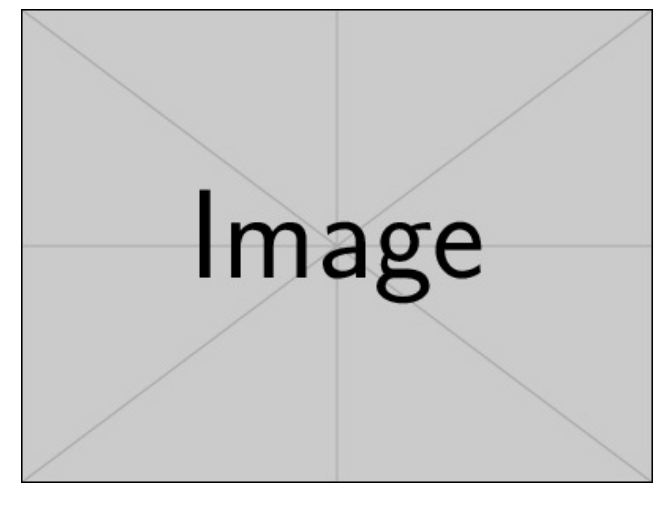
\includegraphics[width=0.5\textwidth]{figures/sample_image.png}
    \caption{A floating figure that may move to an optimal position in the document.}
    \label{fig::floating_figure}
\end{figure}

\begin{color}{gray}
  \lipsum[1]  % Placeholder text to show how figures float
  \lipsum[2]	contenidos...
\end{color}


\subsection{Figures with Black Boxes and Captions}

The following is an example of how to insert a figure with a black box around it, including a caption.

\begin{figure}[H]
    \centering
    \fbox{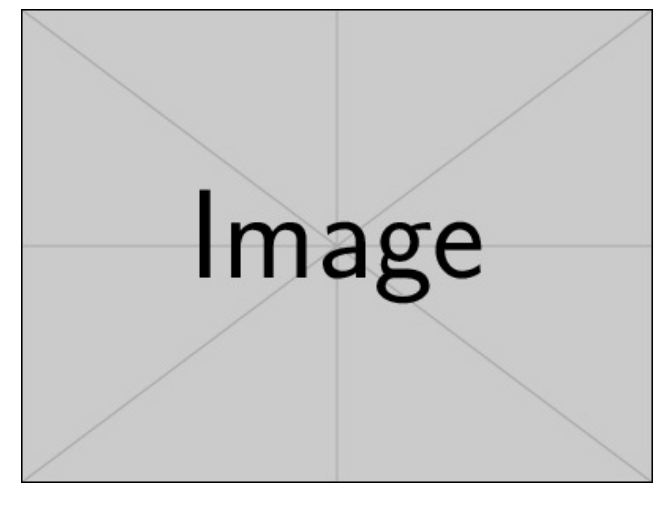
\includegraphics[width=0.6\textwidth]{figures/sample_image.png}}
    \caption{This is a sample figure inside a black box. Captions should be informative and concise.}
    \label{fig::sample_figure}
\end{figure}

This figure uses the `fbox` command to place a black border around the image, and the `caption` package allows you to customize the figure's caption.


\subsection{Wrapping Text Around Figures}

You can also wrap text around a figure, which is helpful when you want to integrate an image into your text without breaking the flow.

\begin{wrapfigure}{R}{0.4\textwidth}
    \centering
    \fbox{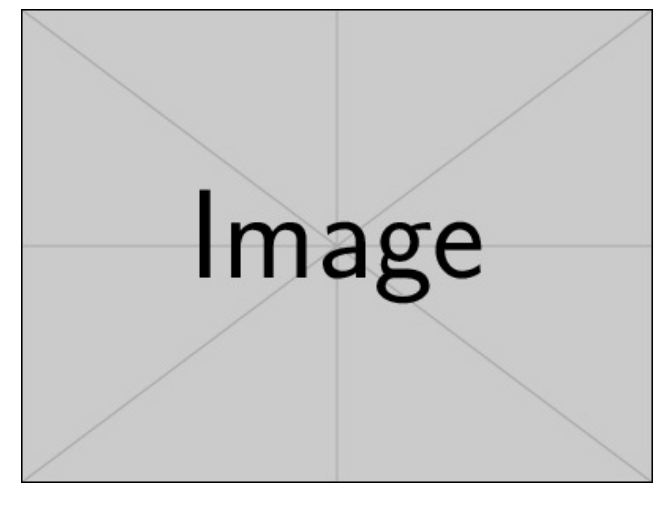
\includegraphics[width=0.38\textwidth]{figures/sample_image.png}}
    \caption{Text wrapped around this figure.}
    \label{fig::wrap_figure}
\end{wrapfigure}

\begin{color}{gray}
  \lipsum[4-6]
\end{color}

The `wrapfig` package allows text to flow around figures, which can enhance the layout of your document when integrating images, as in the figure \ref{fig::wrap_figure}.

\subsection{Mathematical Formulas}

Mathematical expressions can be written in both inline and display style. Here are some examples:

Inline formula: $E = mc^2$.

Display-style formula:

\[
\sum_{i=1}^n i = \frac{n(n+1)}{2}
\]

A more complex equation involving integrals:

\[
\int_{0}^{\infty} e^{-x^2} \, dx = \frac{\sqrt{\pi}}{2}
\]

\subsection{List Structures}

LaTeX supports various types of lists, including unordered, ordered, and description lists.
Unordered list:
\begin{itemize}
    \item First item
    \item Second item
    \item Third item
\end{itemize}
List with bullet point changed:
\renewcommand\labelitemi{\ding{117}}
\begin{itemize}
	\item First item
	\item Second item
	\item Third item
\end{itemize}
Ordered list:
\begin{enumerate}
    \item Step 1
    \item Step 2
    \item Step 3
\end{enumerate}
Description list:
\begin{description}
    \item[Term 1] Definition of the first term.
    \item[Term 2] Definition of the second term.
\end{description}

\subsection{Citations and References}

In academic writing, citations are crucial. Below is an example of a citation using a bibliography entry.

You can cite references in the text like this: \cite{fakeauthor2022article}, \cite{fakeauthor2021book}, \cite{fakeauthor2020conference}, \cite{fakeauthor2019report}, \cite{fakeauthor2018thesis}, \cite{fakeauthor2021website}, \cite{fakeauthor2022github}, \cite{fakeauthor2017chapter}, \cite{fakeauthor2023workshop}, \cite{fakeauthor2020manual}.

\begin{paragraph}{Run-in Heading:}
This is an example of a paragraph with a table on it:
\begin{table}[htbp]
	\begin{center} {\footnotesize
			\begin{tabularx}{\textwidth}{@{} lXlX @{} }
				\multicolumn{2}{c}{} \\ 
				\hline
				
				\normalsize \textbf{Category} & \normalsize \textbf{Description} \\
				
				\hline
				& \\
				Example 1 & Lorem ipsum dolor sit amet, consectetur adipiscing elit. Phasellus bibendum est ut lacus bibendum, non fermentum ex ultricies. Praesent id ipsum sed elit ultricies facilisis. Fusce posuere odio ac tortor gravida, a viverra nibh pretium. \\
				& \\
				Example 2 & Lorem ipsum dolor sit amet, consectetur adipiscing elit. Integer ac nisl eget nulla ultrices venenatis. Vestibulum ante ipsum primis in faucibus orci luctus et ultrices posuere cubilia curae. Donec euismod orci et turpis malesuada, in posuere nisl euismod. \\
				& \\
				Example 3 & Lorem ipsum dolor sit amet, consectetur adipiscing elit. Aliquam sed justo sit amet nisi interdum sodales. Nam eget augue eu sapien scelerisque tempor. Curabitur tincidunt turpis vitae dolor consectetur, ut accumsan erat feugiat. Vestibulum ante ipsum primis in faucibus orci luctus et ultrices posuere cubilia curae. \\
				\hline
		\end{tabularx}}
	\end{center}
	\caption{\footnotesize Example table multicolum}
	\label{tab::example_table_multicolumn}
\end{table}
\end{paragraph}

\subsection{Subsection with icon \icon{figures/sample_image.png}}
Finally, this is an example how to place an icon in a subsection title.

\section{What is LATEX?}
LATEX (pronounced "Lah-tech" or "Lay-tech") is a macro package created by Leslie Lamport based on TEX. As a document preparation system for high-quality typesetting in almost any forms of publishing, LATEX is not the name of a particular editing program, but refers to the encoding or tagging conventions that are used in LATEX documents.

\section{Why use LATEX?}
There are many good reasons to use LATEX. The most significant ones are:
\begin{itemize}
	\item It allows you to clearly separate the content from the format of your document.
	\item It lets you concentrate on your ideas, not the visual appearance.
\end{itemize}

\section{How to use?}
\subsection{Installation}
LaTeX is based on open-source code, so it is available on most platforms as free software. Depending on your operating system, you may encounter different installation instructions.

\begin{itemize}
	\item \textbf{Linux:} TeXLive distribution.
	\item \textbf{MacOS:} MacTeX or TeXLive.
	\item \textbf{Windows:} MiKTeX or TeXLive.
\end{itemize}

\section{How to write the introduction}
The introduction is a crucial section of any research paper, as it establishes the writing style, research quality, and credibility of the author. It provides readers with the necessary background and context to understand the importance of the research being presented. This section begins by broadly introducing the research topic and then narrows down to a specific research question or hypothesis. 

According to the San José State University Writing Center \cite{SJSUWritingCenterIntroduction}, the introduction serves to answer three fundamental questions: (1) What is the research about? (2) Why is it important? (3) What does the author want the reader to understand? 

A well-structured introduction starts with a general overview of the topic, supported by recent research, and gradually becomes more focused, leading to the specific research problem. The introduction should avoid going too in-depth, as detailed analyses are reserved for the body of the paper. Instead, it highlights the research focus, problem statement, and objectives, aligning with the standards of the discipline. Furthermore, it is essential to differentiate between the introduction and the literature review, as the latter critically evaluates existing research, while the introduction sets the stage for the study \cite{SJSUWritingCenterIntroduction}.

In various academic disciplines, the introduction may differ in tone, structure, and content. For instance, in business and engineering, clarity and conciseness are paramount, while in the humanities, there is more room for creativity in presenting the research problem \cite{SJSUWritingCenterIntroduction}. Regardless of the field, a well-crafted introduction should follow a clear organizational structure, often visualized as an inverted triangle, beginning with broad context and narrowing to specific research questions. 

The San José State University Writing Center recommends utilizing the Create a Research Space (CARS) model, which involves three steps: (1) establishing the relevance of the topic, (2) identifying gaps or limitations in existing research, and (3) filling those gaps with the research question, hypothesis, or objectives \cite{SJSUWritingCenterIntroduction}. By following this model, the introduction effectively conveys the significance of the research and guides the reader toward understanding its purpose and scope.


%--------------CHAPTER 2-------------------%
\setcounter{chapter}{1}
\chapter{Related work} \label{relatedWork}

\section{How to write the related work section}
In preparing a related work section, a strategic approach can greatly reduce the time spent searching and reading while maximizing the depth and relevance of the literature. According to Animatas \cite{Animatas2023}, the key steps involve identifying seed papers, expanding and filtering the pool, and finally organizing the related work in a meaningful way.

The process begins by identifying a few initial seed papers, typically from Google Scholar, which serve as a foundation. These papers are added to a spreadsheet, where essential details such as title, authors, and inclusion status are tracked. The next step involves expanding the pool by reviewing citations in the seed papers and adding any relevant ones from the last three years. This expanded list is then filtered by reading abstracts and titles, while noting down reasons for exclusion \cite{Animatas2023}.

Once a core set of relevant papers is identified, the author extracts important keywords from the papers to construct search queries for platforms like Web of Science and Scopus. This helps ensure comprehensive coverage of the literature. The filtered results are carefully documented in the spreadsheet, and the process continues until a solid overview of the literature is achieved. Citation alerts are set up to remain up-to-date with new developments throughout the project \cite{Animatas2023}.

The final step involves organizing the related work section by clustering papers into similar topics, creating brief summaries for each, and weaving them into cohesive paragraphs. This structured approach ensures that the related work section is well-informed and demonstrates how the current research builds on or addresses gaps in previous work \cite{Animatas2023}.


%--------------CHAPTER 3-------------------%

\setcounter{chapter}{2}
\chapter{Proposed Method} \label{chap::proposedMethod}
\section{How to write the proposed method section}
The methodology section outlines how the research was conducted and provides the necessary details for readers to assess the validity and reliability of the study. According to the San José State University Writing Center \cite{SJSUWritingCenterProposedMethod}, this section should describe the research question, the type of data used, and why this data is appropriate for the research. It also involves explaining the data collection process, including the tools, materials, sampling criteria, and the size of the sample.

In quantitative research, the methodology section includes the types of mathematical analyses conducted, whereas qualitative research focuses on identifying patterns in language, theme, or structure from non-numerical data. Additionally, it is important to justify the selected methodology by explaining why it is suitable for the research question and by addressing any challenges encountered \cite{SJSUWritingCenterProposedMethod}.

For the proposed research, data collection involved [insert your data collection methods, e.g., gathering audio-visual data], followed by the implementation of [insert specific tools or technologies used, e.g., machine learning models, audio processing tools]. The criteria for selecting data sources focused on [insert criteria]. The data analysis process involved [insert analysis methods, such as statistical techniques or qualitative coding], ensuring that the analysis aligned with the research objectives. Tools such as [insert tools, e.g., Python, TensorFlow] were used for data processing and interpretation.


%--------------CHAPTER 4-------------------%


\setcounter{chapter}{3}
\chapter{Experiments and Results} \label{chap::experimentsResult}
\section{How to write the experiment and result section}
The results section is a key component of any research paper, as it presents the findings of the study in response to the research question(s). According to the San José State University Writing Center \cite{SJSUWritingCenterResults}, the purpose of this section is to provide the data in a structured and unbiased manner, without attempting to analyze or interpret it. The results can be presented in text, tables, or figures, but the data should always be connected to the research question to maintain relevance.

In presenting the results, it is crucial to follow a logical structure, often organizing the findings either thematically or chronologically. Each set of findings should be clearly introduced to keep the reader’s focus aligned with the study's objectives. Visual aids such as tables and graphs can be used to enhance the presentation but should not replace the textual description of the results \cite{SJSUWritingCenterResults}. 

An effective results section concludes by summarizing the key findings, preparing the reader for the subsequent discussion section, where the implications of the results are analyzed. By adhering to this structure, the results are conveyed clearly and effectively, providing a solid foundation for further interpretation \cite{SJSUWritingCenterResults}.


%--------------CHAPTER 5-------------------%
\setcounter{chapter}{4}
\chapter{Discussion and Future Lines} \label{chap::disscusionFutureLines}
\section{How to write the discussion}
The discussion section is an essential part of the research paper, where the author analyzes, interprets, and explains the findings in relation to the research question(s). According to the San José State University Writing Center \cite{SJSUWritingCenterDiscussion}, the purpose of this section is to place the results in context, explain their significance, and address any unexpected findings. Furthermore, it is important to acknowledge the study's limitations and suggest areas for future research.

An effective discussion begins by summarizing the key findings and linking them to the research question. The findings are then compared with the existing literature to demonstrate how they align or diverge from previous studies. Any unexpected results should be discussed and explained, as they may provide new insights into the research problem. Limitations of the study, such as data constraints or methodological weaknesses, should be transparently addressed to enhance the credibility of the research \cite{SJSUWritingCenterDiscussion}.

In terms of future research, it is essential to propose follow-up studies that can further explore gaps identified in the current research. These recommendations should be concise and focused on the most pressing questions that remain unanswered. Concluding the discussion, the key findings and their broader implications are restated, underscoring the importance of the research in contributing to the field and suggesting potential practical applications \cite{SJSUWritingCenterDiscussion}.


%--------------CHAPTER 6-------------------%
\setcounter{chapter}{5}
\chapter{Conclusion} \label{chap::conclusion}
\section{How to write the conclusion}
The conclusion is a critical component of any research paper, as it is the final opportunity to leave a lasting impression on the reader. According to the San José State University Writing Center \cite{SJSUWritingCenterConclusion}, a well-written conclusion should restate and synthesize the main points of the paper, but without simply repeating what has already been said. Instead, the focus should be on emphasizing how the research has contributed to the reader’s understanding of the topic.

A strong conclusion adds significance to the discussion by connecting the findings to the real world, offering insights into the broader implications of the research. Furthermore, it is important to answer the "So what?" question, explaining why the research matters and how it affects the field or related areas. This ensures that the reader understands the relevance and practical applications of the work \cite{SJSUWritingCenterConclusion}.

Finally, the conclusion may include a call to action or a powerful closing statement that leaves a lasting impact. This can be achieved by summarizing the key contributions of the paper and proposing future steps, ensuring that the research remains memorable and meaningful for the audience \cite{SJSUWritingCenterConclusion}.


\newpage
\nocite{*}
\bibliographystyle{unsrt} 
\bibliography{references} \label{chap::Bibliography}


%--------------ANEXO-------------------%
\chapter*{Anexo}
\section*{Example pyhthon code 1}\label{anexo1}
\begin{lstlisting}[language=Python]

import os

class ThesisTemplate:
	def __init__(self, author_name):
		self.author_name = author_name

	def print_greeting(self):
		message = f"Hello, World! I am a template for the thesis authored by {self.author_name}."
		border = "*" * len(message)
		print(border)
		print(message)
		print(border)

if __name__ == "__main__":
	author = "Your Name"  # Replace with your actual name
	template = ThesisTemplate(author)
	template.print_greeting()
\end{lstlisting}


\section*{Example pyhthon code 2}\label{anexo2}
\begin{lstlisting}[language=Python]
import random
import numpy as np

class SampleTemplate:
	def __init__(self):
		self.operation = self.generate_random_operation()

	def generate_random_operation(self):
		# Generate two random integers
		num1 = random.randint(1, 10)
		num2 = random.randint(1, 10)
		
		# Choose a random operation 
		operations = ['+', '-', '*', '/']
		operation = random.choice(operations)
		
		# Calculate result based on operation
		if operation == '+':
		result = num1 + num2
		elif operation == '-':
		result = num1 - num2
		elif operation == '*':
		result = num1 * num2
		elif operation == '/':
		# Prevent division by zero
		if num2 == 0:
		num2 = 1  # Change num2 to 1 to avoid division by zero
		result = num1 / num2
		
		return f"{num1} {operation} {num2} = {result}"

	def greet(self):
		print("Hello World! I am a template for the thesis.")
		print("Here's a random numeric operation for you:")
		print(self.operation)

# Example of how to use the class
if __name__ == "__main__":
	template = SampleTemplate()
	template.greet()
	


\end{lstlisting}

\end{document}
%---------------------------------------------------------------------------%

